\subsection{Dataset}
    For training the object detection system we use the Open Images Dataset V4 \cite{openImages}, available at \cite{openImagesSite}. In total, the dataset contains 9.2 million images, including 14.6 million bounding boxes across 600 classes on 1.74 million images. We use only a subset of classes: bus, car, and license plate or vehicle registration plate as it is called in the original dataset. 
    
    The tool used to download the bus, car, and license plate classes and the corresponding bounding boxes is OIDv4 ToolKit \cite{OIDv4_ToolKit}. The dataset is split into three parts: train (77.81\%), validation (19.54\%), and test (2.65\%).
    
    The dataset, as it is in its original form, is unbalanced. The car class has around 5-6 times the number of bounding boxes the other classes have. This is problematic because the object detector tends to predict mostly cars.
    
    We try to address this issue by using a technique called undersampling. The idea is that we try to balance the numbers by removing instances of the dominant class.
    
    We further improve the dataset by enhancing the license plate class using an existing highly performant license plate detector. Therefore, we use an object detector based on YOLO \cite{license_plate_enhancer} in order to add new bounding boxes if they don't already exist, because we observed that license plates are not annotated in a lot of images. We can see in Fig. \ref{enhanced_distribution}, the number of boxes and images for each class, and in Table. \ref{enhanced_dataset} we can see the detailed distribution. In total, we have added 3108 license plate bounding boxes to the dataset.

    
%    Another detail is that the maximum number of bounding boxes an image can have is 111.
    
    
    Each image is resized so that its dimension is $416 \times 416$ and the bounding boxes are scaled accordingly. This is done using linear interpolation.
     
    The resizing helps the object detection task, as explained in \cite{yolov2} because this way we can split the image into a grid of $13 \times 13$ cells of size $32 \times 32$ pixels so that there is a cell in the center that can detect the larger objects that are centered in the middle, rather than have 4 cells in the middle that try to detect the same object.
    
    Each image is associated with multiple bounding boxes and each cell is responsible for detecting multiple bounding boxes through the use of anchors as explained in \cite{yolov2}. We use three anchors per cell so that each cell can detect various shapes and sizes. The anchor boxes are chosen using K-Means over the dataset.

    
    For computing the distance between the centroid and bounding box the following formula is used, as in \cite{yolov2}:
    
    \begin{gather*}
        distance(centroid, box) = 1-IOU(centroid, box)
    \end{gather*}
    
    \begin{table}[!b]
    \centering
    \caption{Bounding box statistics related to the undersampled and enhanced subset of Open Images}
    \begin{tabular}{|c|c|cccc|}
    \hline
    \multirow{2}{*}{} & \multirow{2}{*}{No. images} & \multicolumn{4}{c|}{No. bounding boxes}                                                    \\ \cline{3-6} 
                      &                                   & \multicolumn{1}{c|}{Total} & \multicolumn{1}{c|}{Bus} & \multicolumn{1}{c|}{Car} & License plate \\ \hline
    Train      & 19773 & \multicolumn{1}{c|}{50110} & \multicolumn{1}{c|}{11927} & \multicolumn{1}{c|}{28159} & 10024 \\ \hline
    Validation & 4967  & \multicolumn{1}{c|}{10824} & \multicolumn{1}{c|}{92}    & \multicolumn{1}{c|}{9381}  & 1351  \\ \hline
    Test              & 669                               & \multicolumn{1}{c|}{1580}  & \multicolumn{1}{c|}{353} & \multicolumn{1}{c|}{764} & 463           \\ \hline
    \end{tabular}
    \label{enhanced_dataset}
    
    \end{table}
    
    
    Where IOU represents intersection over union between the centroid and the bounding box.
    
   %\begin{figure}[!b]
%      \centering
%      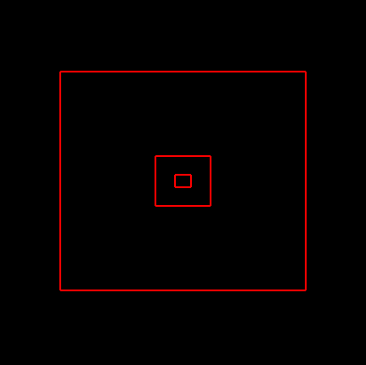
\includegraphics[scale=0.25]{images/anchors_3.png}
%    \caption{Anchors for the bus, car, and license plate classes}
%     \label{3_anchors}
%    \end{figure} 
    
    
    %We have tried to use three, four and five centroids, or clusters, in order to generate the anchors, but in all cases the outer boxes are the same and in the case of four and five anchors, only smaller and smaller anchors are added which are not different enough from each other, therefore we choose to use the variant with three anchors.% represented in Fig. \ref{3_anchors}. 
    
            
   \begin{figure}[!t]
      \centering
      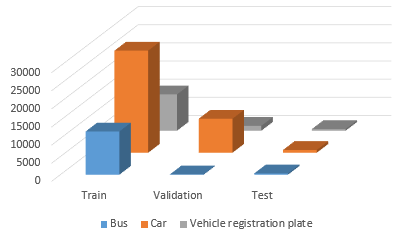
\includegraphics[scale=0.5]{images/enhanced_dataset.png}
      \caption{Undersampled and enhanced dataset bounding boxes distribution}
      \label{enhanced_distribution}
    \end{figure} 
    
    Each image needs to be associated with a ground truth. We represent the ground truth as a $C \times C \times B \times (5+N)$ tensor. For each cell in the $C \times C$ grid, we associate B anchor boxes. Each anchor box has the following parameters: $b_x$ and $b_y$ represent the center of the box, $b_w$ and $b_h$ represent the width and height, c is the probability that the anchor predicts an object and $c_1, c_2, c_3, ... c_n$ represent the class probabilities. In our case, C is 13 and both B and N are 3. Therefore, the output is a tensor of shape $13 \times 13 \times 3 \times 8$.
    
    The formulas that are used to compute the center, width, and height from the output of the model are:
    
    \begin{equation}
    \begin{split}
        & b_x = \sigma(t_x) + c_x \\
        & b_y = \sigma(t_y) + c_y \\
        & b_w = p_w \cdot e^{t_w} \\ 
        & b_h = p_h \cdot e^{t_h}
    \end{split}
    \label{conversion_formulas}
    \end{equation}
    
    Where $t_x, t_y, t_w, t_h$ represent the raw predictions to which the sigmoid function is applied, $c_x, c_y$ represent the coordinates of the upper left corner of the cell that predicts the box, and $p_w, p_h$ represent the width and height of the anchor that predicts the box. Over the output for the class probabilities, the softmax function is applied.
    
    
    